\documentclass{beamer}
\usepackage[utf8]{inputenc}

\usepackage{color}
\usepackage{xcolor}
\definecolor{PLB}{rgb}{0.06,0.42,0.60}
\definecolor{PLBfonce}{rgb}{0.06,0.42,0.60}
\definecolor{PLBmoyen}{RGB}{176, 216, 232}
\definecolor{PLBpale}{rgb}{0.94,0.965,0.965}

%\usetheme{PaloAlto}
\usetheme{Madrid}
\setbeamercolor{frametitle}{bg=PLB}     %controls the color of the headline
\setbeamercolor{sidebar}{bg=PLB}        %controls the color of the sidebar
\setbeamercolor{logo}{bg=PLB!70!black}
\setbeamercolor{structure}{fg=PLB, bg=PLB!40}
%\setbeamertemplate{footline}[default]

\usepackage{amssymb}
\usepackage{pifont}
\usepackage{bigints}
\usepackage{mathrsfs}

\definecolor{mblue}{rgb}{0.18,0.21,0.67}
\definecolor{mgree}{rgb}{0.,0.6,0.}
\definecolor{dgreen}{rgb}{0.,0.6,0.}
\definecolor{violet}{RGB}{142, 68, 173}
\definecolor{bleu}{RGB}{41, 128, 185}
\definecolor{gris}{rgb}{0.5,0.5,0.5}
\newcommand{\cmark}{{\color{dgreen}\ding{52}}}
\newcommand{\xmark}{{\color{red}\ding{55}}}
\newcommand{\bmark}{{\color{orange}$\sim$}}
\newcommand{\arrow}{{\color{PLB}\ding{220}}}
\newcommand{\mbold}[1]{{\textbf{\color{PLB}#1}}}

\usepackage{soul}
\usepackage{multicol}
\usepackage{multirow}

\usepackage{enumitem}
%\setlist[description]{leftmargin=0.5cm}


\usepackage{amsmath}
\usepackage{cancel}
\DeclareMathOperator*{\argmax}{argmax}
\DeclareMathOperator*{\argmin}{argmin}
\DeclareMathOperator\erfi{erfi}

\usepackage[backend=bibtex, style=authoryear-comp]{biblatex}
\usepackage{filecontents}
\renewbibmacro*{cite}{%
  \iffieldundef{shorthand}
    {\ifthenelse{\ifnameundef{labelname}\OR\iffieldundef{labelyear}}
       {\usebibmacro{cite:label}%
        \setunit{\printdelim{nonameyeardelim}}}
       {\printnames{labelname}%
        \setunit{\printdelim{nameyeardelim}}}%
     \usebibmacro{cite:labeldate+extradate}%
     \setunit{\addcomma\space}%
     \usebibmacro{journal}}
    {\usebibmacro{cite:shorthand}}}
\newcommand{\customcite}[1]{\cite{#1}}

\bibliography{biblio}

\beamertemplatenavigationsymbolsempty

%for backup slides
\newcommand{\backupbegin}{
  \newcounter{finalframe}
  \setcounter{finalframe}{\value{framenumber}}
}
\newcommand{\backupend}{
  \setcounter{framenumber}{\value{finalframe}}
}


\AtBeginSection[
  {\frame<beamer>{\frametitle{Outline}   
    \tableofcontents[currentsection,currentsection]}}%
]%
{
  \frame<beamer>{ 
    \frametitle{Outline}   
    \tableofcontents[currentsection,currentsection]}
}

\title[Canum-J 2020]{Exponential methods for solving hyperbolic problems with application to kinetic equations}

\author[J. Massot]{N. Crouseilles \inst{1,2} \and L. Einkemmer \inst{3} \and \underline{J. Massot} \inst{2,1}}
\institute[IRMAR]{\inst{1} Inria Rennes -- Bretagne Atlantique \and \inst{2} IRMAR, Université de Rennes \and \inst{3} University of Innsbruck}
\date{December 4, 2020}

\begin{document}

\begin{frame}[plain]
  \titlepage
\end{frame}

\begin{frame}{Outline}
  \tableofcontents
\end{frame}


\section{Motivation for Vlasov-Poisson equations}
%%%%%%%%%%%%%%%%%%%%%%%%%%%%%%%%%%%%%%%%%%%%%%%%%%%%%%%%%%%%%%%%%%%%%%%%%%%%%%%

\begin{frame}{Vlasov-Poisson equations 1D$\times$1D}
  Our model: a non-linear transport in $(x,v)\in\Omega\times\mathbb{R}$ of an electron density distribution $f=f(t,x,v)$:
  $$
    \begin{cases}
      \partial_t f + v\partial_x f + E\partial_v f = 0 \\
      \partial_x E = \int_{\mathbb{R}} f\,\mathrm{d}v - 1
    \end{cases}
  $$

  \textbf{\color{mblue} Motivation:}
  \begin{itemize}
    \item We want high order methods in $(x,v)$
    \item We want high order methods in time $t$:
      \begin{itemize}
        \item Splitting methods: could have a lot of steps
        \item Runge-Kutta methods: stability constraints (CFL condition)
          \begin{itemize}
            \item The most restrictive CFL condition is associated with the linear part ($\partial_tf + v\partial_x f=0$)
          \end{itemize}
      \end{itemize}
    \end{itemize}
    \arrow We want to propose a compromise: exponential integrators.
\end{frame}
%-------%
\begin{frame}{Vlasov-Poisson equations 1D$\times$1D}
  Fourier transform in $x$ direction of Vlasov, amenable to exponential integrators:
  $$
    \partial_t\hat{f} + ikv\hat{f} + \widehat{E\partial_v f} = 0
  $$
  
  Vlasov is of the form:
  $$
    \dot{u} = iau + F(u)
  $$
  Variation of constant: $\partial_t(e^{-iat}u) = e^{-iat}F(u)$. No more CFL in $x$ of the form $\Delta t\leq \sigma\frac{\Delta x}{v_\text{max}}$ with $[-v_\text{max},v_\text{max}]\equiv\mathbb{R}$.

  Time integration:
  $$
    u(t_n+\Delta t) = \exp(ia\Delta t)u(t_n) + \int_0^{\Delta t}\exp(ia(\Delta t-s))F(u(t_n+s))\,\mathrm{d}s
  $$
  with $\Delta t>0$, $t_n = n\Delta t$ with $n\in\mathbb{N}$

  Linear part is exact! \cmark
\end{frame}
%-------%
\begin{frame}{Idea of exponential integrators}
  \textbf{\color{mblue} 2 classes of methods:}
  \begin{description}[leftmargin=0.25cm]
    \item[\mbold{exponential Runge-Kutta:}] solve exactly what we can, and interpolate the rest. For example first order exponential Euler method:
      $$
        u(t_n+\Delta t) \approx u^{n+1} = e^{-ia\Delta t}u^n + \Delta t\varphi_1(ia\Delta t)F(u^n)
      $$
      where $\varphi_1(z) = \dfrac{e^z - 1}{z}$
      \vspace{-0.1cm}
      \begin{thebibliography}{9}
        \setbeamertemplate{bibliography item}[article]
        \bibitem{a} \customcite{Hochbruck:2010}
      \end{thebibliography}
    \item[\mbold{Lawson:}] Change of variable: $v(t)=e^{-iat}u(t)$, we solve with a RK method: $\dot{v} = \tilde{F}(t,v) = e^{-iat}F(e^{iat}v(t))$

      For example, Lawson Euler method:
      $$
        v(t_n+\Delta t)\approx v^{n+1} = v^n + \Delta t e^{-iat_n}F(e^{iat_n}v^n)
      $$
      or as an expression of $u$:
      $$
        u^{n+1} = e^{-ia\Delta t}u^n + \Delta te^{ia\Delta t}F(u^n)
      $$
      \vspace{-0.75cm}
      \begin{thebibliography}{9}
        \setbeamertemplate{bibliography item}[article]
        \bibitem{a} \customcite{Isherwood:2018}
      \end{thebibliography}
  \end{description}
\end{frame}

\section{Linear analysis}
%%%%%%%%%%%%%%%%%%%%%%%%%%%%%%%%%%%%%%%%%%%%%%%%%%%%%%%%%%%%%%%%%%%%%%%%%%%%%%%
\begin{frame}{Reminder of stability tools}
  \only<1>{
    If we want to study stability of:
    $$
      \partial_t u + \partial_x u = 0
    $$
    with centered scheme (CD2) $(\partial_xu)_j \approx \frac{1}{2\Delta x}(u_{j+1}-u_{j-1})$. After a Fourier transform (\emph{von Neumann analysis}):
    $$
      \dot{u} + i\frac{\sin(k\Delta x)}{\Delta x}u = 0
    $$
    Explicit Euler method in time: we have to stretch \mbold{eigenvalues} (or \mbold{Fourier symbol}) of CD2 into explicit Euler \mbold{stability domain}.
  } \only<2>{
    \begin{figure}\centering
      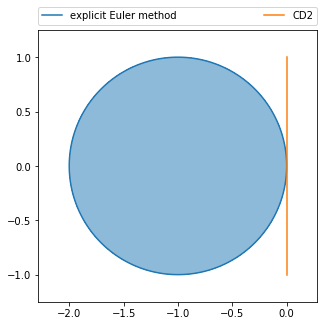
\includegraphics[height=0.8\textheight]{img/cfl_example.png}
    \end{figure}
  }
\end{frame}
%-------%
\begin{frame}{From linear Vlasov equation to toy model}
  Linear Vlasov equation:
  $$
    \partial_t f + a\partial_x f + b\partial_v f = 0
  $$
  Fourier transform in $x$, CD2 in $v$ plus a Fourier transform in $v$, formally:
  $$
    \frac{\mathrm{d}f}{\mathrm{d}t} + iak f + b\frac{i\sin(\varphi)}{\Delta x}f = 0
  $$
  \mbold{Toy model:}
  $$
    \dot{u} + iau + \lambda u = 0
  $$
  with $a\in\mathbb{R}$, $\lambda\in\mathbb{C}$ (diffusive scheme for example).

  $\lambda$ is the Fourier symbol (or eigenvalues) of FD method to approximate $\partial_vf$.
\end{frame}
%-------%
\begin{frame}{Phase space discretization}
  In $v$ direction we use a FD method:
  \begin{itemize}
    \item CD2 (centered difference of order 2): $(\partial_v f)(v_j)\approx \dfrac{f_{j+1}-f_{j-1}}{2\Delta v}$
    \item WENO5 (weighted essentially non-oscillatory of order 5):
      \begin{itemize}
        \item WENO5: non linear scheme: \st{Von Neumann analysis}
        \item LW5 (linearized WENO5): linear scheme (this is Lagrange interpolation of order 5)
      \end{itemize}
      $$
        (\partial_vf)(v_j)\approx\frac{1}{\Delta v}\left(-\frac{1}{30}f_{j-3} + \frac{1}{4}f_{j-2} - f_{j-1} + \frac{1}{3}f_j + \frac{1}{2}f_{j+1} - \frac{1}{20}f_{j+2}\right)
      $$

\begin{thebibliography}{9}
  \setbeamertemplate{bibliography item}[article]
  \bibitem{Wang:2007} \customcite{Wang:2007}
  \bibitem{Motamed:2010} \customcite{Motamed:2010}
\end{thebibliography}

  \end{itemize}
\end{frame}
%-------%
\begin{frame}{Fourier symbols}
  \begin{figure}\centering
    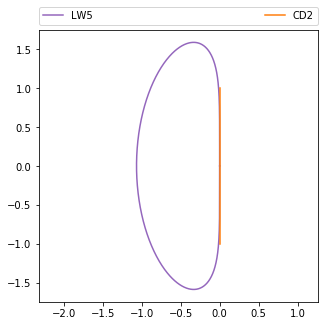
\includegraphics[height=0.8\textheight]{img/weno.png}
  \end{figure}
\end{frame}

\subsection{Lawson methods}
%------------------------------------------------------------------------------
\begin{frame}{Lawson methods stability domain}
  For our toy model:
  $$
    \dot{u} = iau + \lambda(u)
  $$
  Change of variable: $v(t) = e^{-iat}u(t)$
  $$
    \dot{v} = e^{-iat}\lambda e^{iat}v
  $$
  Apply a Runge-Kutta method to compute stability function of Lawson method:
  $$
    v^{n+1} = \underbrace{p(\lambda\Delta t)}_{\text{stability function of RK}}v^n
  $$
  \emph{i.e.}:
  $$
    u^{n+1} = \overbrace{p(\lambda\Delta t)e^{-ia\Delta t}}^{\text{stability function of Lawson}}u^n
  $$
  Stability domain: $\mathcal{D}=\left\{z\in\mathbb{C},|p(z)|\leq 1\right\}$ of Lawson method is \textbf{the same} as the underlying Runge-Kutta method \textbf{because} $ia\in i\mathbb{R}$
\end{frame}
%-------%
\begin{frame}{Considered $Lawson(RK(s,p))$ methods}
  \begin{figure}\centering
    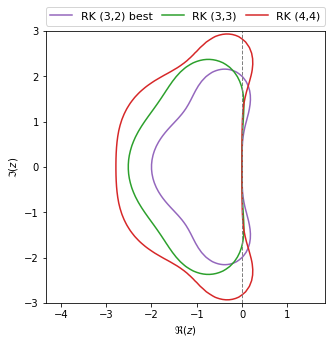
\includegraphics[height=0.75\textheight]{img/rk_sd.png}
    \caption{$\{z\in\mathbb{C},|p(z)|=1\}$}
  \end{figure}
\end{frame}
%-------%
\begin{frame}{Lawson methods -- CD2}
  For stability between a Lawson method and CD2, we solve:
  $$
    |p(iy)| = 1,\quad y\in\mathbb{R}
  $$
  \begin{figure}\centering
    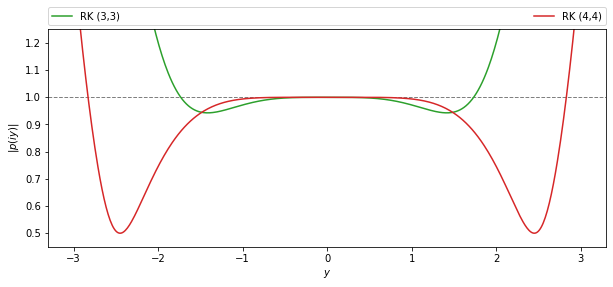
\includegraphics[width=0.8\textwidth]{img/yaxis.png}
  \end{figure}
\end{frame}
%-------%
\begin{frame}{Lawson methods -- LW5}
  \begin{columns}
    \begin{column}{0.5\textwidth}
      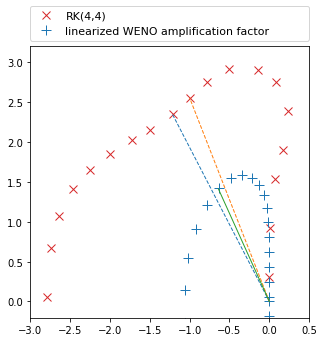
\includegraphics[width=\textwidth]{img/cfl_scheme}
    \end{column}
    \begin{column}{0.5\textwidth}
      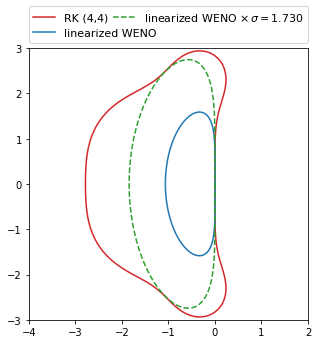
\includegraphics[width=\textwidth]{img/cfl_rk44_weno.png}
    \end{column}
  \end{columns}
\end{frame}
%-------%
\begin{frame}{Lawson methods -- CD2/LW5: CFL estimates}
  \begin{table}
    \centering
    \begin{tabular}{|c|c|c|c|}
      \hline
      - & Lawson($RK(3,3)$) & Lawson($RK(4,4)$) \\
      \hline
      CD2 ($y_{\max}$) & $\sqrt{3}$ & $2\sqrt{2}$\\
      \hline
      LW5 ($\sigma$) & $1.433$   & $1.73$   \\
      \hline  
    \end{tabular}
    \caption{CFL number for some Lawson schemes.}
  \end{table}
  Other RK--CD2 CFL estimates:
\begin{thebibliography}{9}
  \setbeamertemplate{bibliography item}[article]
  \bibitem{} \customcite{Baldauf:2008}
\end{thebibliography}
  Same results for RK--WENO CFL estimates:
\begin{thebibliography}{9}
  \setbeamertemplate{bibliography item}[article]
  \bibitem{} \customcite{Motamed:2010}
  \bibitem{} \customcite{Lunet:2017}
\end{thebibliography}
\end{frame}

\subsection{Exponential Runge-Kutta methods}
%------------------------------------------------------------------------------

\begin{frame}{Exponential Runge-Kutta methods}
  $$
    \dot{u} = iau + F(u)
  $$
  Example on ExpRK(2,2):
  $$
    \begin{aligned}
      u^{(1)} &= e^{-ia\Delta t}u^n - \Delta t\varphi_1 F(u^n) \\
      u^{n+1} &= e^{-ia\Delta t}u^n - \Delta t\left[ (\varphi_1-\varphi_2)F(u^n) + \varphi_2F(u^{(1)}) \right] 
    \end{aligned}
  $$

  Stability function becomes:
  $$
    p_{\text{ExpRK(2,2)}}(z) = \frac{1}{2}\varphi_1\varphi_{1,2}z^2 + (\varphi_1+i\frac{\varphi_1\varphi_{1,2}}{2}a)z + 1 + i\varphi_1a
  $$

  Stability domain depends of $a\Delta t$\dots \xmark
\end{frame}
%-------%
\begin{frame}{}

  \begin{columns}
    \begin{column}{0.5\textwidth}
      \begin{figure}\centering
        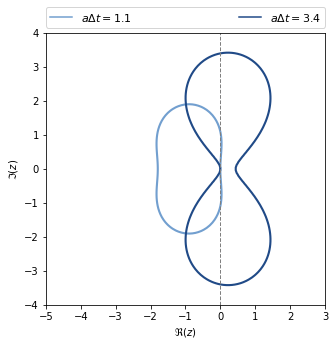
\includegraphics[width=\textwidth]{img/expRK22_sd.png}
        \caption{Stability domain of ExpRK(2,2) for $a\Delta t\in\{1.1, 3.4\}$}
      \end{figure}
    \end{column}
    \begin{column}{0.5\textwidth}
      \begin{figure}\centering
        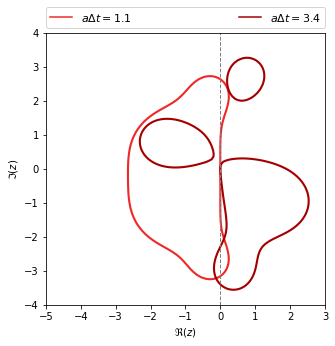
\includegraphics[width=\textwidth]{img/CM_sd.png}
        \caption{Stability domain of Cox-Matthews for $a\Delta t\in\{1.1, 3.4\}$}
      \end{figure}
    \end{column}
  \end{columns}
\end{frame}

\section{Numerical simulation: Vlasov-Poisson equations}
%%%%%%%%%%%%%%%%%%%%%%%%%%%%%%%%%%%%%%%%%%%%%%%%%%%%%%%%%%%%%%%%%%%%%%%%%%%%%%%

\begin{frame}{Vlasov-Poisson equations}
  $$
    \begin{cases}
      \partial_tf + v\partial_xf + E\partial_vf = 0 \\
      \partial_xE = \int_{\mathbb{R}} f\,\mathrm{d}v - 1
    \end{cases}
  $$

  \mbold{Numerical tools:}
  \begin{itemize}
    \item FFT in $x$ direction
    \item CD2 or WENO5 in $v$ direction
    \item $Lawson(RK(s,p))$ method in time $t$
  \end{itemize}

  \mbold{CFL:} $\Delta t_n \leq \dfrac{C\Delta v}{||E^n||_{\infty}} \leq \dfrac{C\Delta v}{\max_n||E^n||_{\infty}}$ where $C = y_\text{max}$ or $\sigma$ from the linear theory.

  \ 

  We can choose: $\Delta t = \min\left( 0.1 , \dfrac{C\Delta v}{\max_n||E^n||_{\infty}} \right)$
\end{frame}
%-------%
\begin{frame}{Landau damping}
  $$
    f(t=0,x,v) = f_0(x,v) = \frac{1}{\sqrt{2\pi}}e^{-\frac{v^2}{2}}(1+0.001\cos(0.5x))
  $$
  $x\in[0,4\pi]$, $v\in[-8,8]$, $N_x = 81$, $N_v=128$

  \ 

  Because of damping:
  $$
    \max_n||E^n||_{\infty} = ||E^0||_\infty
  $$
  So, we choose $\Delta t = 0.1$ (with $\Delta t = 100$ it is still stable!)
\end{frame}
%-------%
\begin{frame}{Landau damping: numerical results}
  \only<1>{
    \begin{figure}
      \centering
      \resizebox{!}{.7\paperheight}{% GNUPLOT: LaTeX picture with Postscript
\begingroup
  \makeatletter
  \providecommand\color[2][]{%
    \GenericError{(gnuplot) \space\space\space\@spaces}{%
      Package color not loaded in conjunction with
      terminal option `colourtext'%
    }{See the gnuplot documentation for explanation.%
    }{Either use 'blacktext' in gnuplot or load the package
      color.sty in LaTeX.}%
    \renewcommand\color[2][]{}%
  }%
  \providecommand\includegraphics[2][]{%
    \GenericError{(gnuplot) \space\space\space\@spaces}{%
      Package graphicx or graphics not loaded%
    }{See the gnuplot documentation for explanation.%
    }{The gnuplot epslatex terminal needs graphicx.sty or graphics.sty.}%
    \renewcommand\includegraphics[2][]{}%
  }%
  \providecommand\rotatebox[2]{#2}%
  \@ifundefined{ifGPcolor}{%
    \newif\ifGPcolor
    \GPcolorfalse
  }{}%
  \@ifundefined{ifGPblacktext}{%
    \newif\ifGPblacktext
    \GPblacktexttrue
  }{}%
  % define a \g@addto@macro without @ in the name:
  \let\gplgaddtomacro\g@addto@macro
  % define empty templates for all commands taking text:
  \gdef\gplbacktext{}%
  \gdef\gplfronttext{}%
  \makeatother
  \ifGPblacktext
    % no textcolor at all
    \def\colorrgb#1{}%
    \def\colorgray#1{}%
  \else
    % gray or color?
    \ifGPcolor
      \def\colorrgb#1{\color[rgb]{#1}}%
      \def\colorgray#1{\color[gray]{#1}}%
      \expandafter\def\csname LTw\endcsname{\color{white}}%
      \expandafter\def\csname LTb\endcsname{\color{black}}%
      \expandafter\def\csname LTa\endcsname{\color{black}}%
      \expandafter\def\csname LT0\endcsname{\color[rgb]{1,0,0}}%
      \expandafter\def\csname LT1\endcsname{\color[rgb]{0,1,0}}%
      \expandafter\def\csname LT2\endcsname{\color[rgb]{0,0,1}}%
      \expandafter\def\csname LT3\endcsname{\color[rgb]{1,0,1}}%
      \expandafter\def\csname LT4\endcsname{\color[rgb]{0,1,1}}%
      \expandafter\def\csname LT5\endcsname{\color[rgb]{1,1,0}}%
      \expandafter\def\csname LT6\endcsname{\color[rgb]{0,0,0}}%
      \expandafter\def\csname LT7\endcsname{\color[rgb]{1,0.3,0}}%
      \expandafter\def\csname LT8\endcsname{\color[rgb]{0.5,0.5,0.5}}%
    \else
      % gray
      \def\colorrgb#1{\color{black}}%
      \def\colorgray#1{\color[gray]{#1}}%
      \expandafter\def\csname LTw\endcsname{\color{white}}%
      \expandafter\def\csname LTb\endcsname{\color{black}}%
      \expandafter\def\csname LTa\endcsname{\color{black}}%
      \expandafter\def\csname LT0\endcsname{\color{black}}%
      \expandafter\def\csname LT1\endcsname{\color{black}}%
      \expandafter\def\csname LT2\endcsname{\color{black}}%
      \expandafter\def\csname LT3\endcsname{\color{black}}%
      \expandafter\def\csname LT4\endcsname{\color{black}}%
      \expandafter\def\csname LT5\endcsname{\color{black}}%
      \expandafter\def\csname LT6\endcsname{\color{black}}%
      \expandafter\def\csname LT7\endcsname{\color{black}}%
      \expandafter\def\csname LT8\endcsname{\color{black}}%
    \fi
  \fi
    \setlength{\unitlength}{0.0500bp}%
    \ifx\gptboxheight\undefined%
      \newlength{\gptboxheight}%
      \newlength{\gptboxwidth}%
      \newsavebox{\gptboxtext}%
    \fi%
    \setlength{\fboxrule}{0.5pt}%
    \setlength{\fboxsep}{1pt}%
\begin{picture}(7200.00,5040.00)%
    \gplgaddtomacro\gplbacktext{%
      \csname LTb\endcsname%%
      \put(814,704){\makebox(0,0)[r]{\strut{}$-18$}}%
      \put(814,1292){\makebox(0,0)[r]{\strut{}$-16$}}%
      \put(814,1880){\makebox(0,0)[r]{\strut{}$-14$}}%
      \put(814,2468){\makebox(0,0)[r]{\strut{}$-12$}}%
      \put(814,3055){\makebox(0,0)[r]{\strut{}$-10$}}%
      \put(814,3643){\makebox(0,0)[r]{\strut{}$-8$}}%
      \put(814,4231){\makebox(0,0)[r]{\strut{}$-6$}}%
      \put(814,4819){\makebox(0,0)[r]{\strut{}$-4$}}%
      \put(946,484){\makebox(0,0){\strut{}$0$}}%
      \put(1678,484){\makebox(0,0){\strut{}$5$}}%
      \put(2410,484){\makebox(0,0){\strut{}$10$}}%
      \put(3142,484){\makebox(0,0){\strut{}$15$}}%
      \put(3875,484){\makebox(0,0){\strut{}$20$}}%
      \put(4607,484){\makebox(0,0){\strut{}$25$}}%
      \put(5339,484){\makebox(0,0){\strut{}$30$}}%
      \put(6071,484){\makebox(0,0){\strut{}$35$}}%
      \put(6803,484){\makebox(0,0){\strut{}$40$}}%
    }%
    \gplgaddtomacro\gplfronttext{%
      \csname LTb\endcsname%%
      \put(308,2761){\rotatebox{-270}{\makebox(0,0){\strut{}$||E(t)||_{L^2}$}}}%
      \put(3874,154){\makebox(0,0){\strut{}$t$}}%
      \csname LTb\endcsname%%
      \put(5816,4646){\makebox(0,0)[r]{\strut{}Lawson$(RK(4,4))$ - WENO5 $\Delta t = 1/8$}}%
      \csname LTb\endcsname%%
      \put(5816,4426){\makebox(0,0)[r]{\strut{}Lawson$(RK(4,4))$ - WENO5 $\Delta t = 1$}}%
      \csname LTb\endcsname%%
      \put(5816,4206){\makebox(0,0)[r]{\strut{}slope $-0.153$}}%
    }%
    \gplbacktext
    \put(0,0){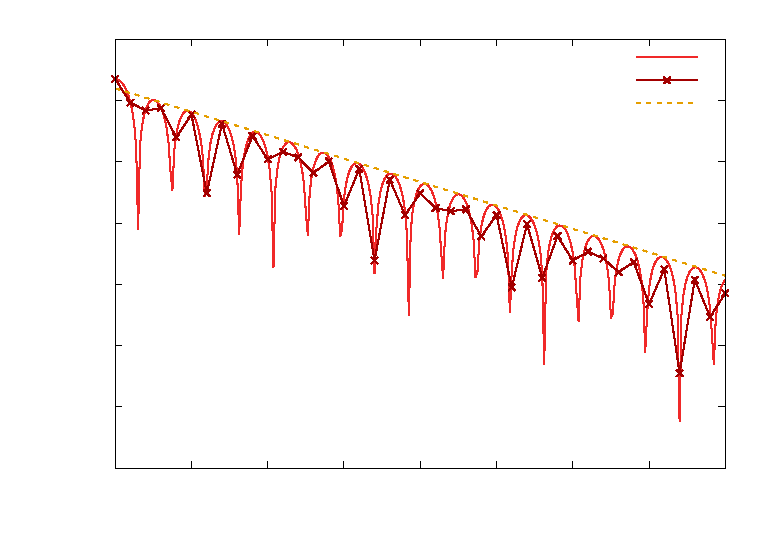
\includegraphics{img/Emax}}%
    \gplfronttext
  \end{picture}%
\endgroup
}
      \caption{Landau damping test: time history of $\|E(t)\|_{L^2}$ (semi-log scale) obtained with Lawson($RK(4, 4)$) and WENO5 
      with $\Delta t=1/8$ and $\Delta t=1$.}
      \label{ld}
    \end{figure}
  }
  \only<2>{
    \begin{figure}
      \centering
      \resizebox{!}{.7\paperheight}{% GNUPLOT: LaTeX picture with Postscript
\begingroup
  \makeatletter
  \providecommand\color[2][]{%
    \GenericError{(gnuplot) \space\space\space\@spaces}{%
      Package color not loaded in conjunction with
      terminal option `colourtext'%
    }{See the gnuplot documentation for explanation.%
    }{Either use 'blacktext' in gnuplot or load the package
      color.sty in LaTeX.}%
    \renewcommand\color[2][]{}%
  }%
  \providecommand\includegraphics[2][]{%
    \GenericError{(gnuplot) \space\space\space\@spaces}{%
      Package graphicx or graphics not loaded%
    }{See the gnuplot documentation for explanation.%
    }{The gnuplot epslatex terminal needs graphicx.sty or graphics.sty.}%
    \renewcommand\includegraphics[2][]{}%
  }%
  \providecommand\rotatebox[2]{#2}%
  \@ifundefined{ifGPcolor}{%
    \newif\ifGPcolor
    \GPcolorfalse
  }{}%
  \@ifundefined{ifGPblacktext}{%
    \newif\ifGPblacktext
    \GPblacktexttrue
  }{}%
  % define a \g@addto@macro without @ in the name:
  \let\gplgaddtomacro\g@addto@macro
  % define empty templates for all commands taking text:
  \gdef\gplbacktext{}%
  \gdef\gplfronttext{}%
  \makeatother
  \ifGPblacktext
    % no textcolor at all
    \def\colorrgb#1{}%
    \def\colorgray#1{}%
  \else
    % gray or color?
    \ifGPcolor
      \def\colorrgb#1{\color[rgb]{#1}}%
      \def\colorgray#1{\color[gray]{#1}}%
      \expandafter\def\csname LTw\endcsname{\color{white}}%
      \expandafter\def\csname LTb\endcsname{\color{black}}%
      \expandafter\def\csname LTa\endcsname{\color{black}}%
      \expandafter\def\csname LT0\endcsname{\color[rgb]{1,0,0}}%
      \expandafter\def\csname LT1\endcsname{\color[rgb]{0,1,0}}%
      \expandafter\def\csname LT2\endcsname{\color[rgb]{0,0,1}}%
      \expandafter\def\csname LT3\endcsname{\color[rgb]{1,0,1}}%
      \expandafter\def\csname LT4\endcsname{\color[rgb]{0,1,1}}%
      \expandafter\def\csname LT5\endcsname{\color[rgb]{1,1,0}}%
      \expandafter\def\csname LT6\endcsname{\color[rgb]{0,0,0}}%
      \expandafter\def\csname LT7\endcsname{\color[rgb]{1,0.3,0}}%
      \expandafter\def\csname LT8\endcsname{\color[rgb]{0.5,0.5,0.5}}%
    \else
      % gray
      \def\colorrgb#1{\color{black}}%
      \def\colorgray#1{\color[gray]{#1}}%
      \expandafter\def\csname LTw\endcsname{\color{white}}%
      \expandafter\def\csname LTb\endcsname{\color{black}}%
      \expandafter\def\csname LTa\endcsname{\color{black}}%
      \expandafter\def\csname LT0\endcsname{\color{black}}%
      \expandafter\def\csname LT1\endcsname{\color{black}}%
      \expandafter\def\csname LT2\endcsname{\color{black}}%
      \expandafter\def\csname LT3\endcsname{\color{black}}%
      \expandafter\def\csname LT4\endcsname{\color{black}}%
      \expandafter\def\csname LT5\endcsname{\color{black}}%
      \expandafter\def\csname LT6\endcsname{\color{black}}%
      \expandafter\def\csname LT7\endcsname{\color{black}}%
      \expandafter\def\csname LT8\endcsname{\color{black}}%
    \fi
  \fi
    \setlength{\unitlength}{0.0500bp}%
    \ifx\gptboxheight\undefined%
      \newlength{\gptboxheight}%
      \newlength{\gptboxwidth}%
      \newsavebox{\gptboxtext}%
    \fi%
    \setlength{\fboxrule}{0.5pt}%
    \setlength{\fboxsep}{1pt}%
\begin{picture}(7200.00,5040.00)%
    \gplgaddtomacro\gplbacktext{%
      \csname LTb\endcsname%%
      \put(990,440){\makebox(0,0)[r]{\strut{}$0.01$}}%
      \put(990,987){\makebox(0,0)[r]{\strut{}$0.1$}}%
      \put(990,1535){\makebox(0,0)[r]{\strut{}$1$}}%
      \put(990,2082){\makebox(0,0)[r]{\strut{}$10$}}%
      \put(990,2629){\makebox(0,0)[r]{\strut{}$100$}}%
      \put(990,3177){\makebox(0,0)[r]{\strut{}$1000$}}%
      \put(990,3724){\makebox(0,0)[r]{\strut{}$10000$}}%
      \put(990,4272){\makebox(0,0)[r]{\strut{}$100000$}}%
      \put(990,4819){\makebox(0,0)[r]{\strut{}$1\times10^{6}$}}%
      \put(1122,220){\makebox(0,0){\strut{}$0$}}%
      \put(1832,220){\makebox(0,0){\strut{}$5$}}%
      \put(2542,220){\makebox(0,0){\strut{}$10$}}%
      \put(3252,220){\makebox(0,0){\strut{}$15$}}%
      \put(3963,220){\makebox(0,0){\strut{}$20$}}%
      \put(4673,220){\makebox(0,0){\strut{}$25$}}%
      \put(5383,220){\makebox(0,0){\strut{}$30$}}%
      \put(6093,220){\makebox(0,0){\strut{}$35$}}%
      \put(6803,220){\makebox(0,0){\strut{}$40$}}%
    }%
    \gplgaddtomacro\gplfronttext{%
      \csname LTb\endcsname%%
      \put(4950,4646){\makebox(0,0)[r]{\strut{}$\frac{\sigma\Delta v}{||E^n||_{L^\infty}}$}}%
      \csname LTb\endcsname%%
      \put(4950,4426){\makebox(0,0)[r]{\strut{}Effective time step}}%
    }%
    \gplbacktext
    \put(0,0){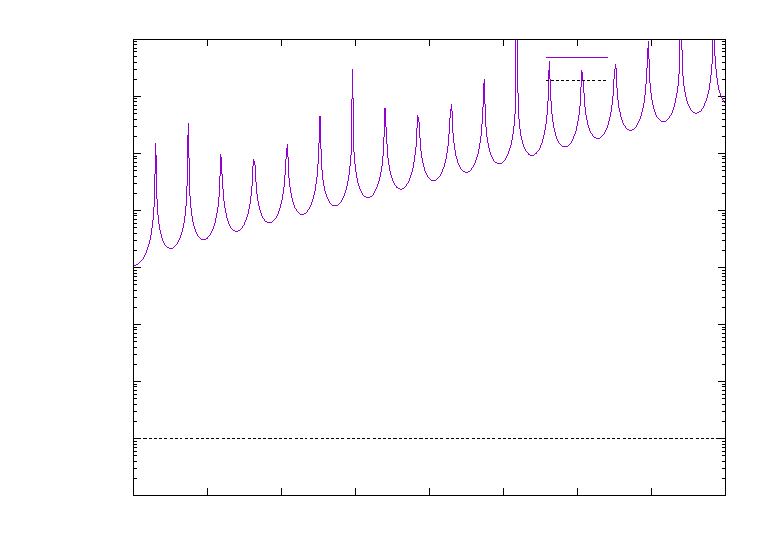
\includegraphics{img/hn}}%
    \gplfronttext
  \end{picture}%
\endgroup
}
      \caption{Landau damping test: time history of the CFL condition (semi-log scale).}
      \label{ld}
    \end{figure}
  }
\end{frame}
%-------%
\begin{frame}{Bump on Tail (BoT)}
  $$
    f(t=0,x,v) = \left[\frac{0.9}{\sqrt{2\pi}}e^{-\frac{v^2}{2}} + \frac{0.2}{\sqrt{2\pi}}e^{-2(v-4.5)^2} \right](1+0.001\cos(0.5x))
  $$

  $x\in[0,20\pi]$, $v\in[-8,8]$, $N_x = 135$, $N_v=256$

  Numerical estimation of $\max_n||E^n||_\infty\approx 0.6$, we choose $\Delta t = \frac{C\Delta v}{0.6}$
\end{frame}
%-------%
\begin{frame}{BoT: numerical results}
  \only<1>{
    \begin{figure}
    \centering
        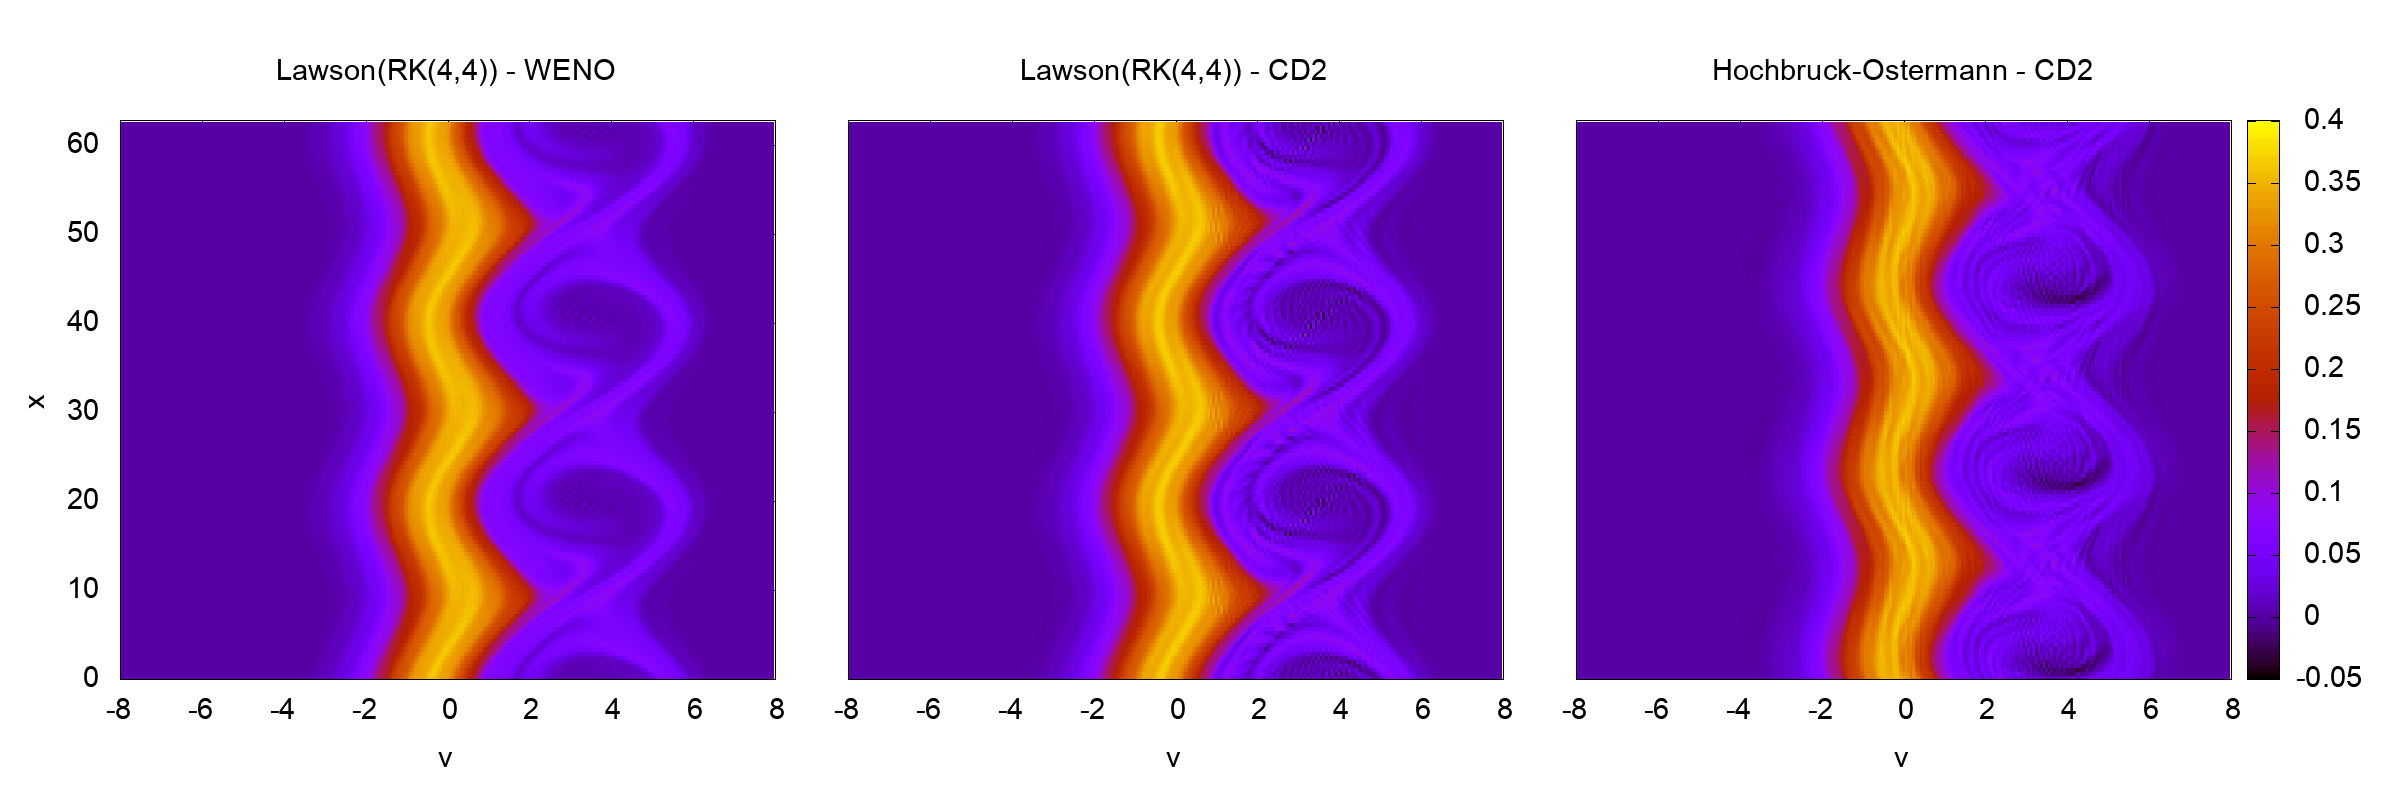
\includegraphics[width=\textwidth]{img/vp_cfl.png}
        \caption{Distribution function at time $t=40$ as a function of $x$ and $v$ for Lawson($RK(4, 4)$) + WENO5 (left), Lawson($RK(4, 4)$) + centered scheme (center), Hochbruck--Ostermann + centered scheme (right).}  
    \label{space}      
    \end{figure}
  } \only<2> {
    \begin{columns}
      \begin{column}{0.5\textwidth}
        \begin{figure}
          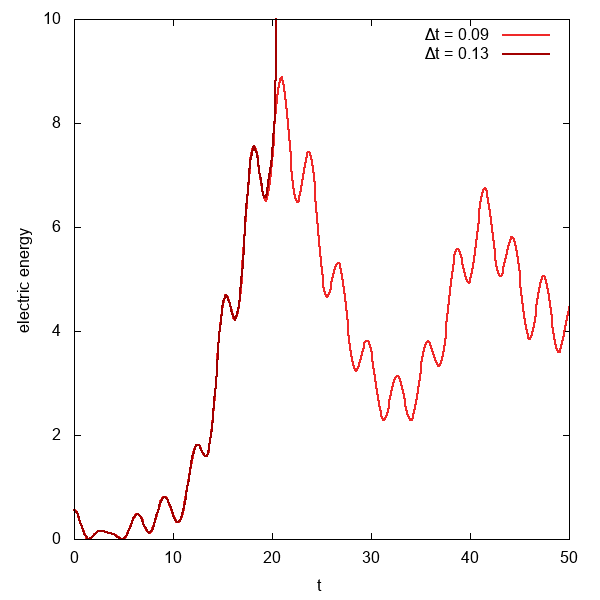
\includegraphics[width=0.9\textwidth]{img/ee_weno_rk44.png}
          \caption{Illustration of the accuracy of the CFL estimate obtained from the linear theory. History of electric energy with Lawson($RK(4,4)$) + WENO5}
        \end{figure}
        \vfill
        \ 
      \end{column}
      \begin{column}{0.5\textwidth}
        \begin{figure}
          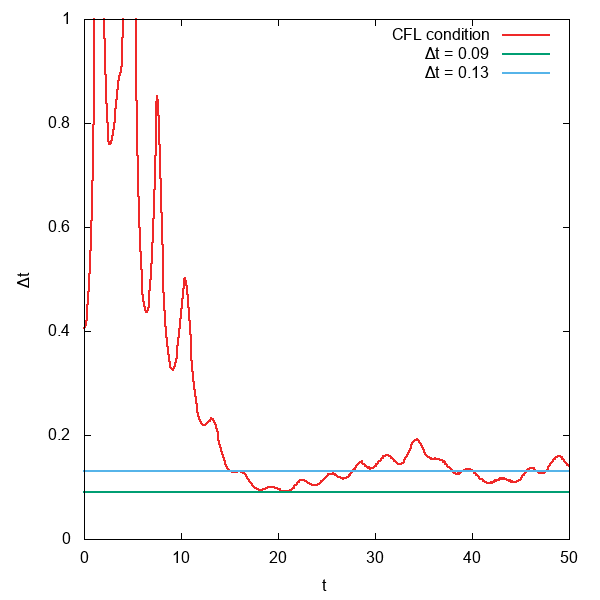
\includegraphics[width=0.9\textwidth]{img/bot_cfl_weno_rk44.png}
          \caption{History of CFL condition for Lawson($RK(4,4)$) + WENO5 case}
        \end{figure}
        \vfill
        \ 
      \end{column}
    \end{columns}
  }
\end{frame}

\section{Conclusion}
%%%%%%%%%%%%%%%%%%%%%%%%%%%%%%%%%%%%%%%%%%%%%%%%%%%%%%%%%%%%%%%%%%%%%

\begin{frame}{Conclusion}
  \mbold{Summary}
  \begin{itemize}
    \item Better understanding on stability of Lawson or ExpRK methods in transport equations
    \item Python script with \texttt{sympy} to compute estimates of CFL of Lawson -- CD2, Lawson -- WENO (5 or 3)
    %\item An adaptive time step size which works with any time integrators
  \end{itemize}

  \mbold{Future works}
  \begin{itemize}
    \item We can improve method with an embedded Runge-Kutta method (Dormand-Prince method, used in \texttt{ode45} of Matlab)
    \item Compare performance between exponential integrators and splitting methods (same order)
    \item Use semi-Lagrangian method to remove dependency on periodic space (Fourier transform)
  \end{itemize}
\end{frame}

\begin{frame}[t]
  \vfill
  {\usebeamerfont{title} Thank you for your attention}
  \vfill
\end{frame}

\appendix
\backupbegin

\begin{frame}[plain]
  \vspace{0.65\textwidth}
  \hfill\footnotesize{Backup}
\end{frame}
%-------%
\begin{frame}{}
\end{frame}


%-------%
\backupend

\end{document}
